% &latex
\documentclass[11pt]{asaproc}

\usepackage{graphicx}
\usepackage{caption}
\usepackage{multirow}
\usepackage{float}
\usepackage{subcaption}
\usepackage{array}
\usepackage{ragged2e}
\usepackage{framed}
\newcolumntype{P}[1]{>{\RaggedRight\hspace{0pt}}p{#1}}

%\usepackage{mathtime}

%%UNCOMMENT following line if you have package
\usepackage{times}

\title{Drivers Of Community Attachment: An Interactive Analysis}

\author{Jessica M. Orth\thanks{Department of Statistics and Actuarial Science, The University of Iowa, 241 Schaeffer Hall Iowa City, IA 52242-1409
}}
\begin{document}
%\SweaveOpts{concordance=TRUE}


\maketitle

\begin{abstract}
In this research, we will investigate several different approaches and
methods to displaying multivariate data. Emphasis will be placed on
end-user-customization tools and flexibility in dynamic and
interactive displays. Specifically, we will highlight the use of
motion charts using Markus Gesmann's \texttt{googleVis} package in R. We will
demonstrate the visualization of time-series data and also the results
of multidimensional scaling and principal component analysis using
this tool. The goals of these displays are ease of usability and
interpretation, dynamic customization options, and the ability to
display multivariate data in a meaningful way. In addition we will
explore partial least squares path modeling using data collected from
the Knight Foundation and Gallup during the years 2008-2010 to
illustrate the attachment of people to their communities in a new and
innovative way.  
\begin{keywords}
Dynamic graphics; Interactive visualizations; Multivariate
statistical analysis 
\end{keywords}
\end{abstract}



\section{Approach}
Displaying multivariate data can be achieved in many ways through a
variety of tools. Here we aim to emphasize the use of motion charts
for displaying the trend analysis of time-dependent Principal
Component Analysis (PCA) and Multidimensional Scaling (MDS). It is well known that
these methods are used as data reduction and data mining techniques in the
analysis of multivariate data, but what happens when we introduce a
time variable to these results? As will be seen, motion charts provide
the tool to seamlessly merge these results throughout time and allow
for dynamic and interactive interpretations of what attaches people to
their communities. 


We analyze the results of 43,000 people from 26 communities across
America using the index variables collected from the `Soul of the
Community' survey conducted by the Knight Foundation and Gallup.  Additional details related to this survey and the Data Expo 2013 can be found in Hofmann (2019). The
cities are shown in Figure 1. Cities are colored based on
the five levels of urbanicity used by the Soul of the Community and
defined by the U.S. Census Bureau as `the percentage of the population
living in urban areas'. The U.S. Census Bureau classifies urban as
`all territory, population, and housing units located within an
urbanized area (UA) or an urban cluster (UC)'. The levels of urbanicity
used by the Soul of the Community are: Very high urbanicity-very large
population, very high urbanicity-large population, very high
urbanicity-medium population, high urbanicity-medium population, and
medium/low urbanicity-low population. The size of the circle for each
city is determined by the log of the total population.

\pagebreak

\begin{figure}[h]
\begin{center}
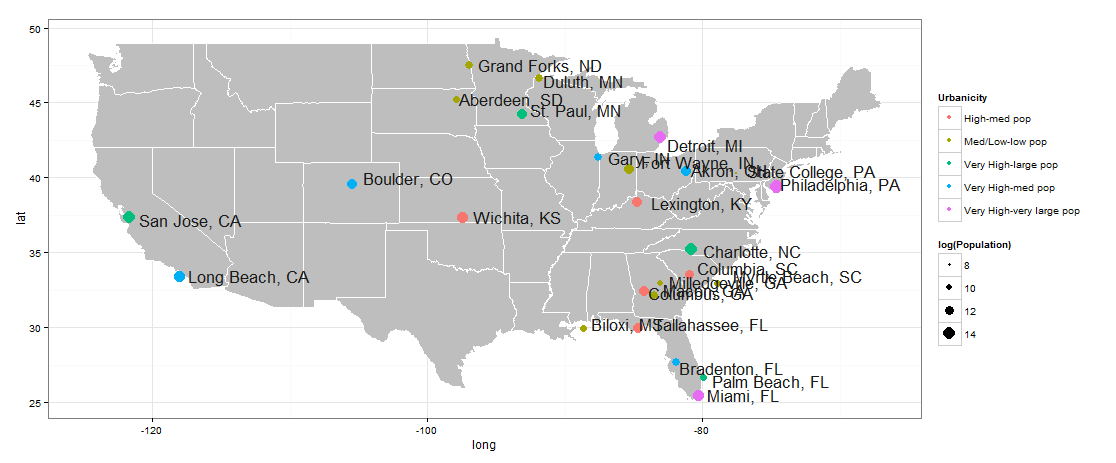
\includegraphics[width=150mm]{map_new.png}
\caption{Locations of communities surveyed.}
\label{fig:map}
\end{center}
\end{figure}


The index variables analyzed include the specific attributes that make people
live where they live such as: attachment, loyalty, passion, basic services,
leadership, education, safety, aesthetics, economy, social offerings,
community offerings, civic involvement, openness, social capital, and
community domains. Our analysis looks at four different summary
statistics: means, standard deviations, the proportion of high index
variables, and z-scores.  


Means, standard deviations, and proportions are calculated for cities
based on the categorical responses on scales of 0-3 and 0-5. The
z-scores serve as an index themselves since they are calculated for
each index variable by city in relation to the collection of responses
for the index variables. This provides information on each
city's score for the original index variables: negative z-scores imply
a lower score for the index variable and positive z-scores indicate a
higher score for that city, relative to the overall score of the
original index variable. 


Data reduction and data mining techniques are applied to these
summary statistics and the results of PCA and MDS are displayed dynamically in
interactive motion charts. To view the motion charts dynamically, see 
\textit{http://mnstats.morris.umn.edu/JSM2013.html}. To view source files for reproducing this research see  
\textit{https://github.com/COSTDataExpo2013}. In Section 2 we investigate how
the index variables are related to each other by identifying the
dynamic drivers that affect community attachment. In
Section 3 we examine the relationships between the
cities and consider clusters of similar cities as well as explore the
movement of dynamic cities throughout the three years
surveyed. Section 4 explores a partial least squares path modeling 
approach to the findings cited by the Knight Foundation and
conclusions and future research are addressed in Section 5. Figure 2 shows a summary of our approach. 

\pagebreak

\begin{figure}[h]
\begin{center}
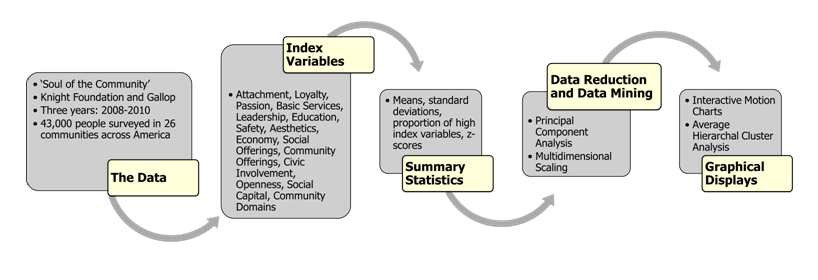
\includegraphics[width=150mm]{chart.png}
\caption{Diagram of our approach.}
\label{fig:chart}
\end{center}
\end{figure}


\section{Key Drivers and Relationships Between Them (PCA)}
PCA seeks to create uncorrelated linear combinations of
the index variables that explain a maximal amount of variation in the
data. In traditional PCA, the set of linear
combinations of the variables with the greatest variance is used as
the first principal component and has the following form: 
\begin{equation}
y_{1} = a_{11}x_{1} + a_{12}x_{2} + \dots + a_{1p}x_{p}
\end{equation}
 with the constraint
that $\mathbf{a_{1}'a_{1}} = 1$. Subsequent principal components are
constructed similarly, with the general form
\begin{equation}
 y_{k} = a_{k1}x_{1} + a_{k2}x_{2} + \dots + a_{kp}x_{p} =
 \mathbf{a_{k}'x}
\end{equation}
 with constraints
$\mathbf{a_{k}'a_{k}} = 1$ and $\mathbf{a_{k}'a_{i}} = 0$ for $(i<k)$.  

We construct time-dependent principal components, taking into account
the three years surveyed, and expressed as
\begin{equation}
 y_{k}(t) = a_{k1}(t)x_{1}(t) + a_{k2}(t)x_{2}(t) + \dots + a_{kp}(t)x_{p}(t) =
 \mathbf{a_{k}(t)'x(t)}
\end{equation}
 with constraints
$\mathbf{a_{k}(t)'a_{k}(t)} = 1$ and $\mathbf{a_{k}(t)'a_{i}(t)} = 0$ for $(i<k)$.




We investigate the first two principal components obtained from the
summary statistics. Tables 1-3 show the loadings from the
analysis. Note the changes in the loadings as we move from Dimension 1
to Dimension 2 throughout time. For the means in Table 1, the loadings are
positive and mostly close to $1$ in Dimension 1, and they change to
mostly negative and closer to $0$ in Dimension 2. In Table 2, we see a contrast
between social capital and safety vs. all other index variables in
Dimension 1 for the standard deviations in 2008, while the contrast in
2009 and 2010 is only between safety and all other index variables for
Dimension 1. The loadings for proportions in Table 3 show a contrast of safety
and aesthetics vs. all other index variables in 2008 for Dimension 1,
while in 2009 the contrast is between social capital vs. all other
index variables. In 2010 we obtain the overall effect of attachment
without contrasts. Leadership in Dimension 2 for proportions in Table
3 changes from
positive to negative to positive throughout the three years, while
economy and openness change from negative to positive to negative. Social
offerings are positive in 2008 and negative in 2009-2010, while
community offerings have the opposite effect. 

The first dimension of the PCA serves as an
index for the overall drivers of attachment for each summary
statistic, while the second dimension shows a contrast between
economic growth and emotional bond. We are able to explain
approximately 55-75\% of the variation in the data with the first two
dimensions.


\begin{table}[h]
\begin{center}
\resizebox{8.65cm}{!}{
%\begin{tabular}{P{3.75cm}P{1.5cm}P{1.5cm}P{1.5cm}|P{1.5cm}P{1.5cm}P{1.5cm}}
\begin{tabular}{P{3.75cm}{r}{r}{r}{r}{r}{r}}
\hline
\hline
& \multicolumn{3}{c}{Dimension 1} & \multicolumn{3}{c}{Dimension 2} \\
\hline
Index Variable & 2008 & 2009 & 2010 & 2008 & 2009 & 2010 \\
\hline
Loyalty & 0.92 & 0.89 & 0.91 & -0.22 & -0.33 & -0.28 \\
Passion & 0.89 & 0.88 & 0.89 & -0.34 & -0.39 & -0.38 \\
Community Attachment & 0.91 & 0.89 & 0.91 & -0.29 & -0.37 & -0.34 \\
Basic Services & 0.28 & 0.36 & 0.43 & 0.50 & 0.34 & 0.12 \\
Leadership & 0.74 & 0.77 & 0.79 & 0.26 & 0.24 & 0.39 \\
Education & 0.72 & 0.77 & 0.83 & 0.46 & 0.38 & 0.31 \\
Safety & 0.49 & 0.62 & 0.70 & 0.65 & 0.61 & 0.53 \\
Aesthetics & 0.57 & 0.67 & 0.74 & -0.14 & -0.21 & -0.28 \\
Economy & 0.66 & 0.69 & 0.81 & -0.02 & 0.11 & 0.31 \\
Social Offerings & 0.72 & 0.79 & 0.80 & -0.40 & -0.39 & -0.38 \\
Community Offerings & 0.94 & 0.96 & 0.98 & 0.24 & 0.17 & 0.13 \\
Involvement & 0.56 & 0.59 & 0.41 & -0.04 & 0.24 & 0.03 \\
Openness & 0.68 & 0.74 & 0.75 & -0.54 & -0.45 & -0.49 \\
Social Capital & 0.49 & 0.42 & 0.48 & 0.70 & 0.73 & 0.74 \\
Domains & 0.96 & 0.97 & 0.98 & -0.01 & 0.07 & 0.01 \\
\hline
\end{tabular}}
\caption{Loadings for PCA on means for survey years 2008-2010.}
\label{table:pcaMeans}
\end{center}
\end{table}

\begin{table}[h]
\begin{center}
\resizebox{8.65cm}{!}{
%\begin{tabular}{P{3.75cm}P{1.5cm}P{1.5cm}P{1.5cm}|P{1.5cm}P{1.5cm}P{1.5cm}}
\begin{tabular}{P{3.75cm}{r}{r}{r}{r}{r}{r}}
\hline
\hline
& \multicolumn{3}{c}{Dimension 1} & \multicolumn{3}{c}{Dimension 2} \\
\hline
Index Variable & 2008 & 2009 & 2010 & 2008 & 2009 & 2010 \\
\hline
Loyalty & 0.41 & 0.54 & 0.50 & 0.83 & 0.78 & 0.81 \\
Passion & 0.41 & 0.50 & 0.46 & 0.84 & 0.80 & 0.80 \\
Community Attachment & 0.46 & 0.54 & 0.50 & 0.85 & 0.80 & 0.81 \\
Basic Services & 0.60 & 0.65 & 0.61 & -0.00 & -0.00 & 0.28 \\
Leadership & 0.67 & 0.56 & 0.43 & -0.50 & -0.55 & -0.69 \\
Education & 0.58 & 0.59 & 0.53 & -0.11 & 0.12 & 0.15 \\
Safety & -0.20 &  -0.17 & -0.32 & 0.18 & -0.18 & 0.04 \\
Aesthetics & 0.70 & 0.65 & 0.64 & 0.29 & 0.35 & 0.43 \\
Economy & 0.30 & 0.41 & 0.24 & -0.65 & -0.67 & -0.83 \\
Social Offerings & 0.70 & 0.65 & 0.72 & -0.42 & -0.48 & -0.38 \\
Community Offerings & 0.94 & 0.91 & 0.86 & -0.14 & -0.28 & -0.20
\\
Involvement & 0.18 & 0.60 & 0.67 & -0.25 & -0.34 & -0.22 \\
Openness & 0.82 & 0.73 & 0.75 & -0.02 & -0.24 & -0.30 \\
Social Capital & -0.02 & 0.40 & 0.45 & 0.38 & 0.52 & -0.00  \\
Domains & 0.63 & 0.83 & 0.68 & -0.23 & -0.31 & -0.53 \\
\hline
\end{tabular}}
\caption{Loadings for PCA on standard deviations for survey years
  2008-2010.}
\label{table:pcaSD}
\end{center}
\end{table}

\begin{table}[h]
\begin{center}
\resizebox{8.65cm}{!}{
%\begin{tabular}{P{3.75cm}P{1.5cm}P{1.5cm}P{1.5cm}|P{1.5cm}P{1.5cm}P{1.5cm}}
\begin{tabular}{P{3.75cm}{r}{r}{r}{r}{r}{r}}
\hline
\hline
& \multicolumn{3}{c}{Dimension 1} & \multicolumn{3}{c}{Dimension 2} \\
\hline
Index Variable & 2008 & 2009 & 2010 & 2008 & 2009 & 2010 \\
\hline
Loyalty & 0.95 & 0.88 & 0.89 & -0.04 & -0.29 &  -0.25 \\
Passion & 0.72 & 0.75 &  0.82 & 0.31 & 0.25 & 0.14 \\
Community Attachment & 0.94 & 0.89 & 0.89 & -0.04 & -0.28 &
-0.26  \\
Basic Services & 0.21 & 0.45 &  0.37 & -0.42 & -0.41 & -0.59 \\
Leadership & 0.73 & 0.77 & 0.85 &  0.02 & -0.06 & 0.05 \\
Education & 0.44 & 0.61 & 0.72 & 0.56 & 0.46 & 0.39 \\
Safety & -0.03 & 0.29 & 0.34 & 0.69 &  0.67 & 0.76 \\
Aesthetics & -0.08 & 0.05 & 0.31 & 0.67 & 0.77 & 0.60 \\
Economy & 0.72 & 0.88 & 0.63 & -0.17 & 0.05 & -0.19 \\
Social Offerings & 0.85 & 0.88 & 0.86 &  0.01 & -0.13 & -0.11 \\
Community Offerings & 0.29 & 0.69 & 0.15 & -0.48 & -0.02 & 0.27 \\
Involvement & 0.18 & 0.27 & 0.55 & 0.83 & 0.58 & 0.27 \\
Openness & 0.62 & 0.46 & 0.31 & -0.29 &  0.12 & -0.50 \\
Social Capital & 0.05 & -0.35 & 0.16 & 0.51 & 0.26 & 0.57 \\
\hline
\end{tabular}}
\caption{Loadings for PCA on proportions for survey years 2008-2010.}
\label{table:pcaProportions}
\end{center}
\end{table}

\pagebreak


 We are interested in the change in the relationship of the
index variables from year to year, and the motion charts clearly show
the dynamic drivers of attachment for each summary statistic. Dynamic
drivers of attachment are those index variables that move between
groups over the course of the three years. These can be seen in
Figures 3-5 and Table
4, but viewed more easily in the interactive
version. 


One of the many beauties of motion charts is the capability to put the
analysis into the hands of the user. Rather than limit a client with
one simple graphical display, motion charts allow for customizable
analyses to suit the interests of multiple users. All one has to do is
change the axes, or modify the color variable or size variable, to
create a unique analysis that is more informative than a single display.


While social offerings, openness, and aesthetics are found to be the
leading drivers of community attachment by the Knight Foundation, we
are able to examine the relationship between these and the other index
variables easily with the motion charts. The first principal component
is plotted on the x-axis and the second principal component on the
y-axis, with the color specified by the index variables. By viewing
the display on the log-log scale, which only changes the axes scale,
we are able to observe two distinct clusters in each of the summary
statistics: overall drivers of attachment and emotional bond. 



The motion charts are shown in stages by year in Figures 3-5 and Table 4
summarizes the clusters of index variables identified by each
statistic in the PCA. While it is easier to view the motion charts
interactively, one is still able to identify the movement of the index
variables between the years in Figures 3-5. 

\begin{figure}[h]
\begin{framed}
\begin{minipage}[b]{0.45\linewidth}
\centering
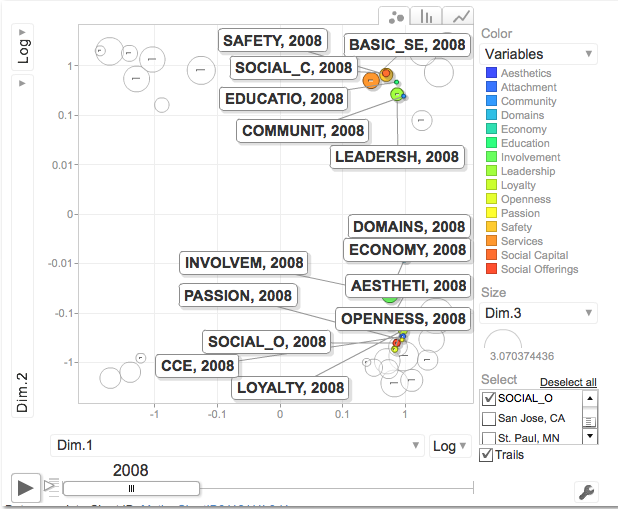
\includegraphics[width=\textwidth]{pcameans08.png}
%\caption{2008}
\end{minipage}
\hspace{0.5cm}
\begin{minipage}[b]{0.45\linewidth}
\centering
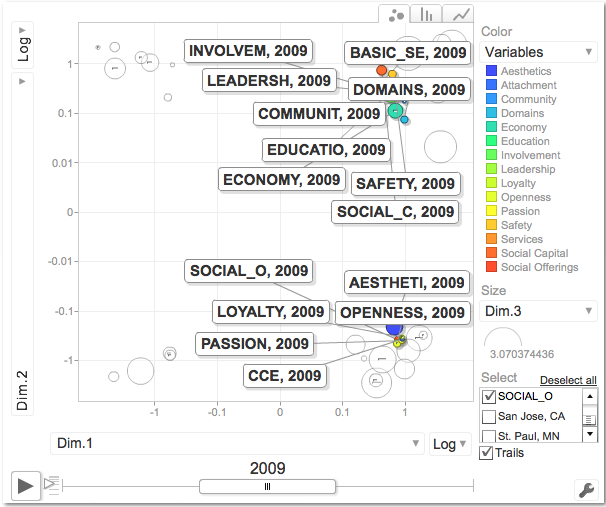
\includegraphics[width=\textwidth]{pcameans09.png}
%\caption{2009}
\end{minipage}
\hspace{0.5cm}
\begin{minipage}[b]{0.45\linewidth}
\centering
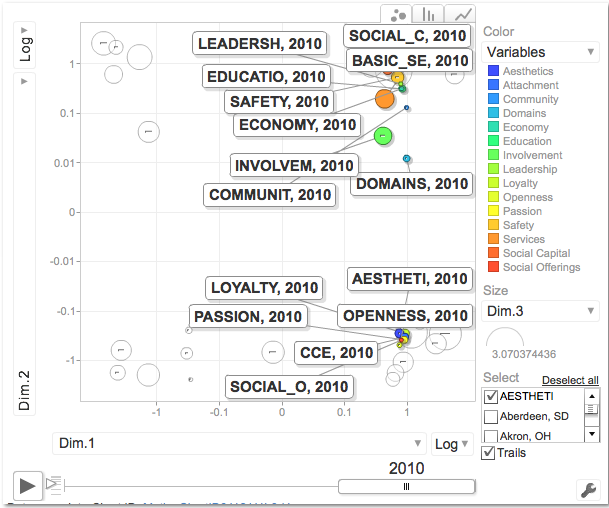
\includegraphics[width=\textwidth]{pcameans10.png}
%\caption{2010}
\end{minipage}
\hspace{0.5cm}
\begin{minipage}[b]{0.45\linewidth}
\centering
%\includegraphics[width=\textwidth]{}
\caption{PCA results of the means for 2008-2010. 
Dimension 1 is on the x-axis and Dimension 2 is on the y-axis. 
The data are shown on the log-log scale, 
with color specified by the index variables.}
\label{fig:pcaMCmeans}
\end{minipage}
\end{framed}
\end{figure}


\begin{figure}[H]
\begin{framed}
\begin{minipage}[b]{0.45\linewidth}
\centering
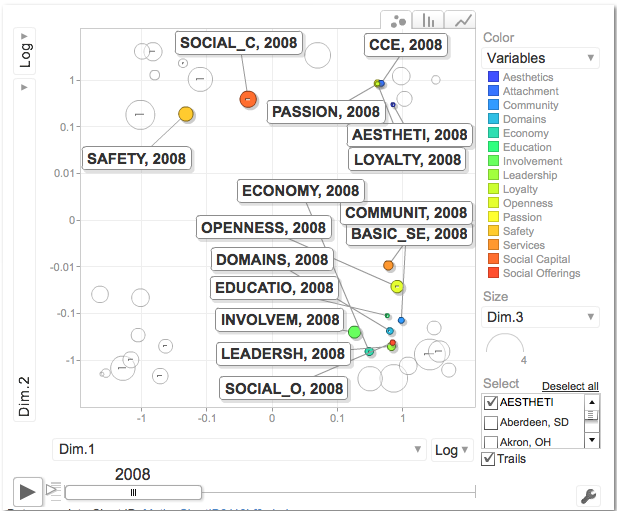
\includegraphics[width=\textwidth]{pcasd08.png}
%\caption{2008}
\end{minipage}
\hspace{0.5cm}
\begin{minipage}[b]{0.45\linewidth}
\centering
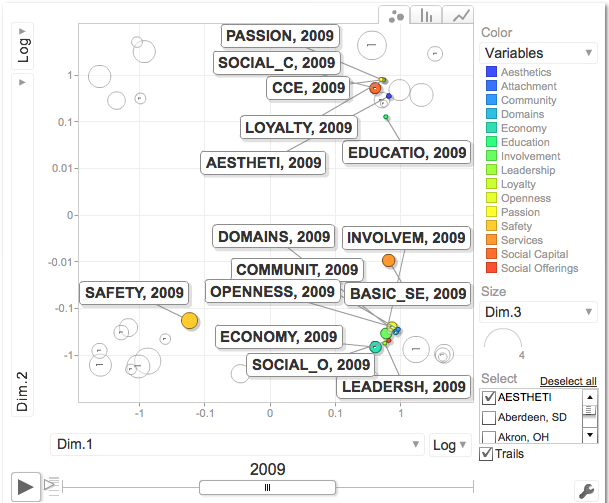
\includegraphics[width=\textwidth]{pcasd09.png}
%\caption{2009}
\end{minipage}
\hspace{0.5cm}
\begin{minipage}[b]{0.45\linewidth}
\centering
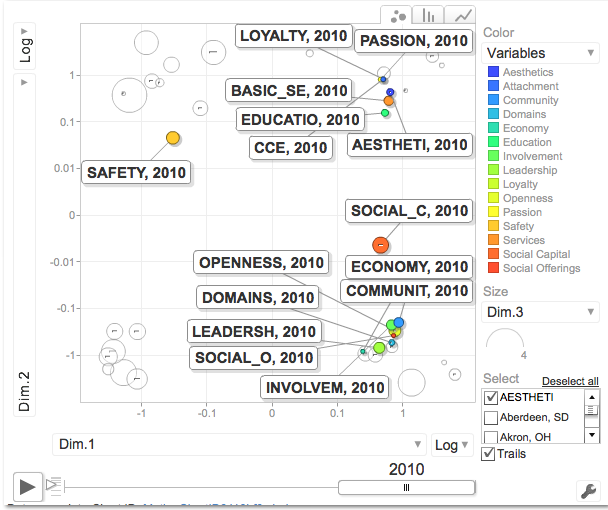
\includegraphics[width=\textwidth]{pcasd10.png}
%\caption{2010}
\end{minipage}
\hspace{0.5cm}
\begin{minipage}[b]{0.45\linewidth}
\centering
%\includegraphics[width=\textwidth]{}
\caption{PCA results of the standard deviations for 2008-2010. Dimension 1 is on the
x-axis and Dimension 2 is on the y-axis. The data are shown on the
log-log scale, with color specified by the index variables.}
\label{fig:pcaMCsd}
\end{minipage}
\end{framed}
\end{figure}

\begin{figure}[ht]
\begin{framed}
\begin{minipage}[b]{0.45\linewidth}
\centering
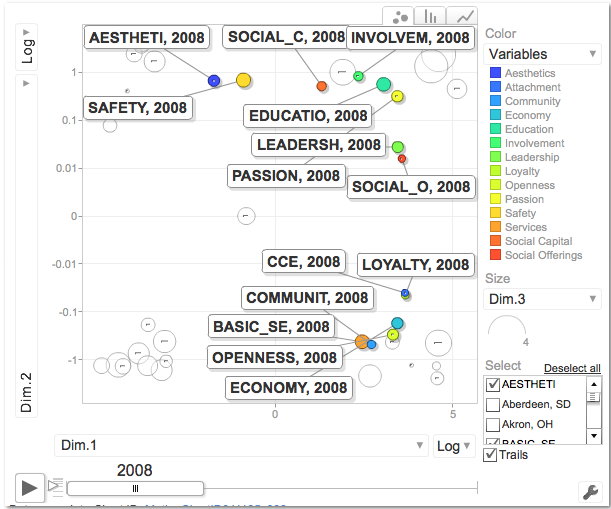
\includegraphics[width=\textwidth]{pcaproportions08.png}
%\caption{2008}
\end{minipage}
\hspace{0.5cm}
\begin{minipage}[b]{0.45\linewidth}
\centering
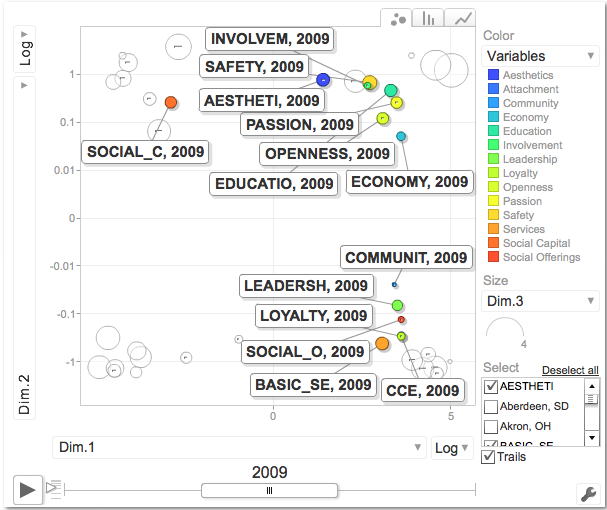
\includegraphics[width=\textwidth]{pcaproportions09.png}
%\caption{2009}
\end{minipage}
\hspace{0.5cm}
\begin{minipage}[b]{0.45\linewidth}
\centering
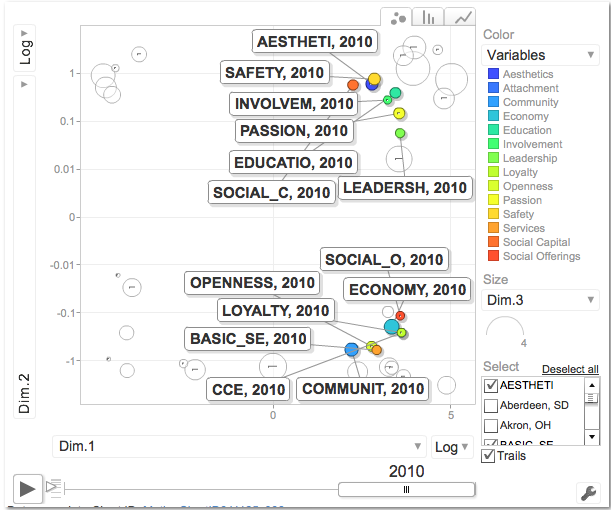
\includegraphics[width=\textwidth]{pcaproportions10.png}
%\caption{2010}
\end{minipage}
\hspace{0.5cm}
\begin{minipage}[b]{0.45\linewidth}
\centering
%\includegraphics[width=\textwidth]{}
\caption{PCA results of the proportions for 2008-2010. Dimension 1 is on the
x-axis and Dimension 2 is on the y-axis. The data are shown on the
log-log scale, with color specified by the index variables.}
\label{fig:pcaMCproportions}
\end{minipage}
\end{framed}
\end{figure}


\pagebreak

\begin{table}
[H]
\begin{center}

\resizebox{10cm}{!}{

\begin{tabular}{P{3cm}P{3cm}P{3cm}P{3cm}}

\hline

\hline
& Means & Standard Deviations & Proportions \\

\hline

Dimension 1    & Overall drivers for attachment & Personal Assurance

vs. Overall drivers for attachment & Personal Assurance vs. Overall

drivers for attachment \\

\hline

Percentage of  & 2008: 54 & 2008: 32 & 2008: 35\\

Variation      & 2009: 58 & 2009: 38 & 2009: 42\\

Explained       & 2010: 62 & 2010: 34 & 2010: 39\\

\hline

\hline

Dimension 2 & Economic Growth vs. Emotional Bond & Personal Assurance

and Pride vs. Economic Growth & Emotional Bond vs. Economic Growth\\

\hline

Percentage of  & 2008: 15 & 2008: 23 & 2008: 20\\

Variation        & 2009: 14 & 2009: 25 & 2009: 15\\

Explained        & 2010: 13 & 2010: 27 & 2010: 20\\

\hline

Dynamic Drivers & Involvement, Economy, Domains & Safety, Social

Capital, Education, Basic Services & Safety, Aesthetics, Social

Capital, Leadership, Social Offering, Openness, Economy\\

\hline

\hline

\end{tabular}}

\caption{Dynamic drivers and percentage of variation explained by
  PCA.}

\label{table:DynamicDrivers}
\end{center}

\end{table}






\section{Differences Between Communities (MDS)}


The goal of MDS is to provide a visual
representation of the pattern of similarities and differences among
the cities. By calculating the Euclidean distance between the points,
MDS maps the cities based on proximity matrices. Let $d_{ij}(t)$
represent the distance between two cities, \emph{i} and \emph{j}, at
time \emph{t} based on their coordinate vectors $\mathbf{x_{i}(t)}$ and
$\mathbf{x_{j}(t)}$ for different time periods. Then the Euclidean
distance is calculated as  
\begin{equation}
d_{ij}(t) = \sqrt{{\sum_{k=1}^d} (x_{ik}(t) - x_{jk}(t))^2}, \  i,j=1,\dots,26
\end{equation}

We use the index variables to determine the relationships
between the cities. Cities estimated to be very similar to each other
in these characteristics are placed close to each other on the map,
and those estimated to be very different from each other are placed
far away from each other on the map. Tables 6-9 in the Appendix show the loadings from the analysis.


Motion charts provide many different ways one can interpret the
clusters and dimensions of the MDS. In Figures
6-9, we can see distinct clusters of cities. We can group them by
region or urbanicity to search for patterns in the clusters. Dynamic
cities, which are those cities that move from cluster to cluster throughout the
years, are marked on the charts. 

Higher mean scores and proportion scores imply that the city scored
higher averaged across all index variables. Dynamic cities with high values in
these summary statistics include: Biloxi MS, Palm Beach FL,
Milledgeville GA, Boulder CO, Tallahassee FL, Aberdeen SD, Grand Forks
ND, Wichita KS, Columbus GA, Long Beach CA, and Myrtle Beach SC. A
higher score in standard deviations implies that the responses for
that city had more variation averaged across the index variables. Dynamic cities with a
high variation in responses include: State College PA, Wichita KS,
Tallahassee FL, Palm Beach FL, Philadelphia PA, and Myrtle Beach SC. Higher
z-scores indicate a higher city score relative to the original index
variables. Columbus is the only dynamic city for the z-scores that
scored higher relative to the original index variables. 

MDS has allowed us to identify not only distinct
clusters of cities that are more similar in their responses to the
index variables, but also detect dynamic cities and observe how the
characteristics of the cities change throughout time. These features
are highlighted in Figures 6-9. 

\begin{figure}[ht]
\begin{framed}
\begin{minipage}[b]{0.45\linewidth}
\centering
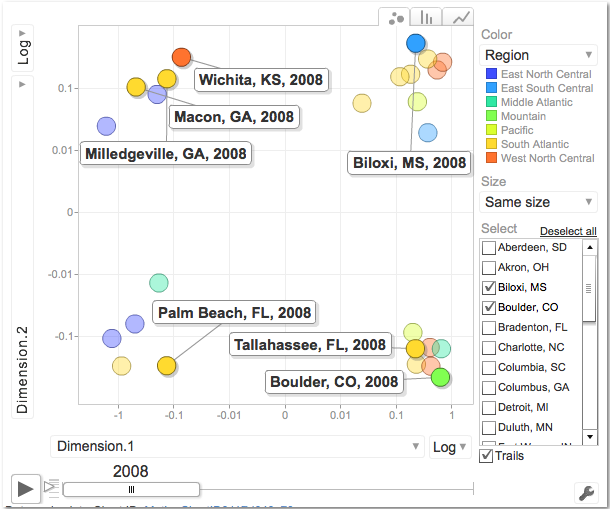
\includegraphics[width=\textwidth]{mdsmeans08.png}
%\caption{2008}
\end{minipage}
\hspace{0.5cm}
\begin{minipage}[b]{0.45\linewidth}
\centering
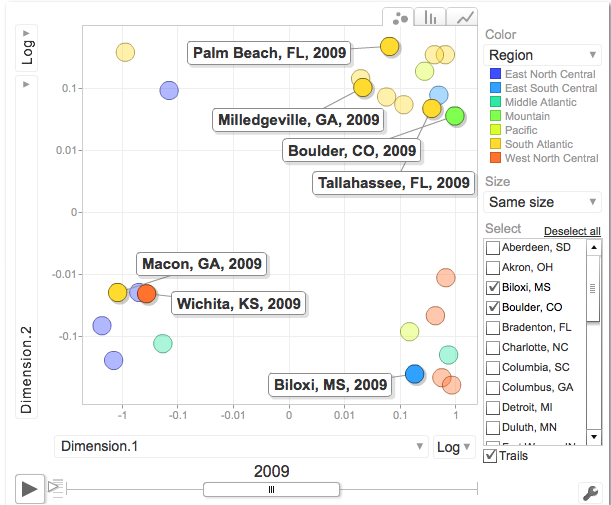
\includegraphics[width=\textwidth]{mdsmeans09.png}
%\caption{2009}
\end{minipage}
\hspace{0.5cm}
\begin{minipage}[b]{0.45\linewidth}
\centering
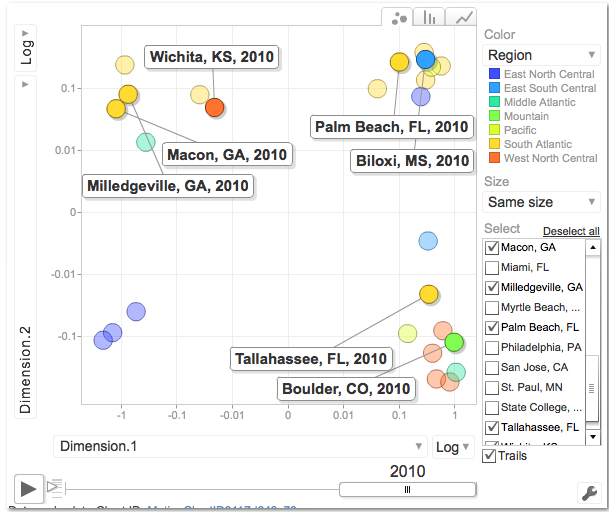
\includegraphics[width=\textwidth]{mdsmeans10.png}
%\caption{2010}
\end{minipage}
\hspace{0.5cm}
\begin{minipage}[b]{0.45\linewidth}
\centering
%\includegraphics[width=\textwidth]{}
\caption{MDS results on the means for 2008-2010. Dimension 1 is on the
  x-axis and Dimension 2 is on the y-axis. The data are shown on the
  log-log scale, with color specified by Region.}
\label{fig:mdsMCmeans}
\end{minipage}
\end{framed}
\end{figure}

\pagebreak

\begin{figure}[H]
\begin{framed}
\begin{minipage}[b]{0.45\linewidth}
\centering
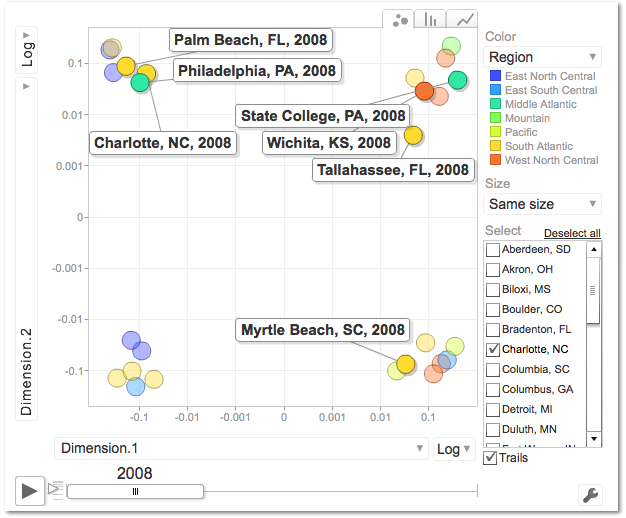
\includegraphics[width=\textwidth]{mdssd08.png}
%\caption{2008}
\end{minipage}
\hspace{0.5cm}
\begin{minipage}[b]{0.45\linewidth}
\centering
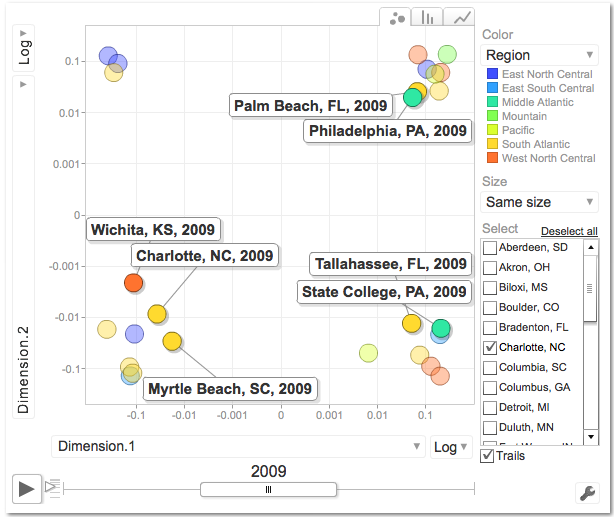
\includegraphics[width=\textwidth]{mdssd09.png}
%\caption{2009}
\end{minipage}
\hspace{0.5cm}
\begin{minipage}[b]{0.45\linewidth}
\centering
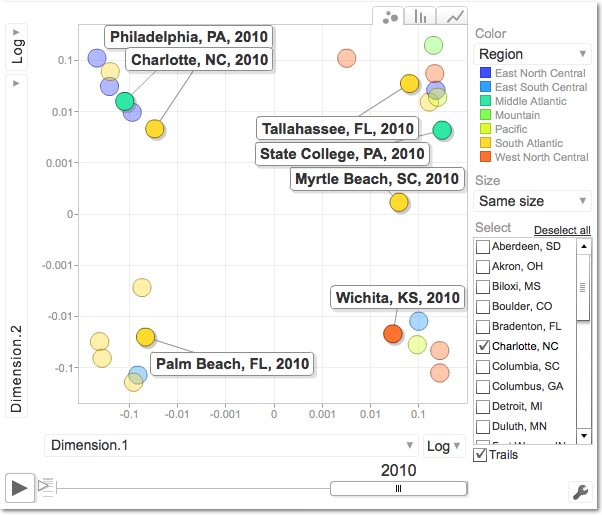
\includegraphics[width=\textwidth]{mdssd10.png}
%\caption{2010}
\end{minipage}
\hspace{0.5cm}
\begin{minipage}[b]{0.45\linewidth}
\centering
%\includegraphics[width=\textwidth]{}
\caption{MDS results on the standard deviations for
  2008-2010. Dimension 1 is on the x-axis and Dimension 2 is on the
  y-axis. The data are shown on the log-log scale, with color
  specified by Region.}
\label{fig:mdsMCsd}
\end{minipage}
\end{framed}
\end{figure}

\begin{figure}[H]
\begin{framed}
\begin{minipage}[b]{0.45\linewidth}
\centering
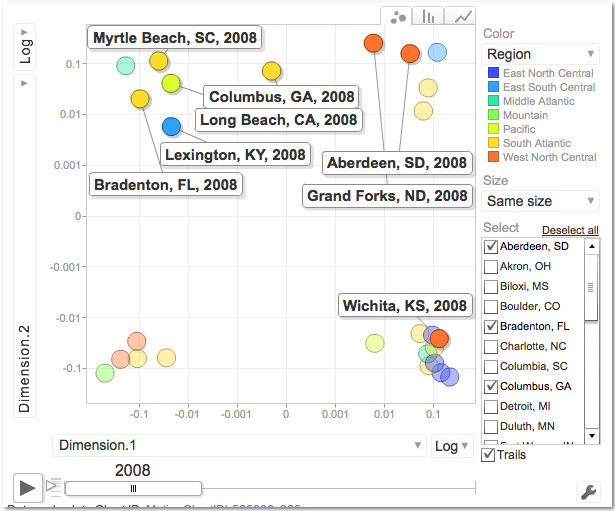
\includegraphics[width=\textwidth]{mdsproportions08.png}
%\caption{2008}
\end{minipage}
\hspace{0.5cm}
\begin{minipage}[b]{0.45\linewidth}
\centering
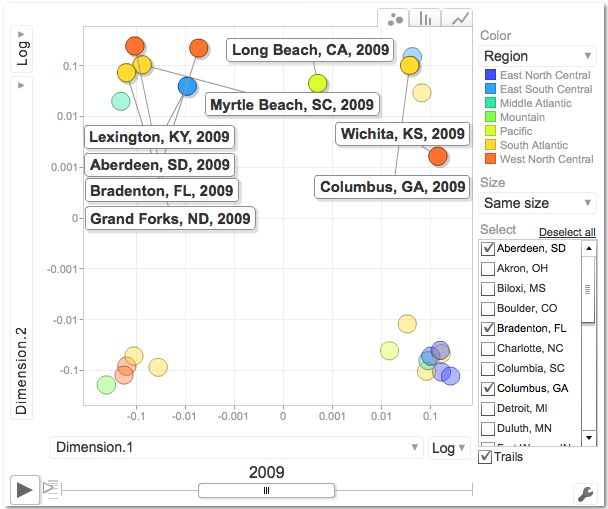
\includegraphics[width=\textwidth]{mdsproportions09.png}
%\caption{2009}
\end{minipage}
\hspace{0.5cm}
\begin{minipage}[b]{0.45\linewidth}
\centering
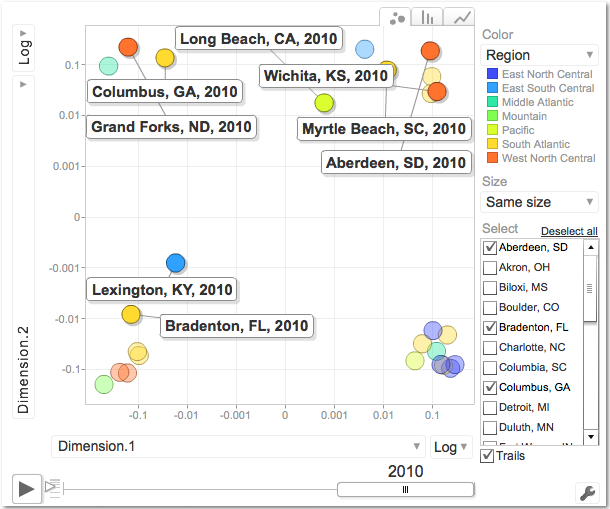
\includegraphics[width=\textwidth]{mdsproportions10.png}
%\caption{2010}
\end{minipage}
\hspace{0.5cm}
\begin{minipage}[b]{0.45\linewidth}
\centering
%\includegraphics[width=\textwidth]{}
\caption{MDS results on the proportions for
  2008-2010. Dimension 1 is on the x-axis and Dimension 2 is on the
  y-axis. The data are shown on the log-log scale, with color
  specified by Region.}
\label{fig:mdsMCproportions}
\end{minipage}
\end{framed}
\end{figure}

\begin{figure}[h]
\begin{framed}
\begin{minipage}[b]{0.45\linewidth}
\centering
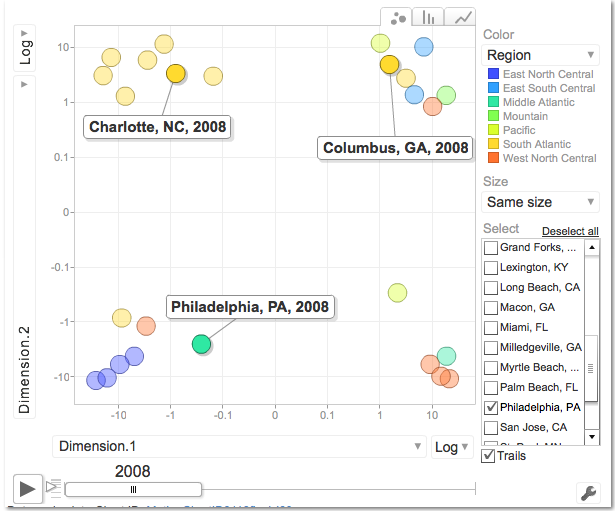
\includegraphics[width=\textwidth]{mdszscores08.png}
%\caption{2008}
\end{minipage}
\hspace{0.5cm}
\begin{minipage}[b]{0.45\linewidth}
\centering
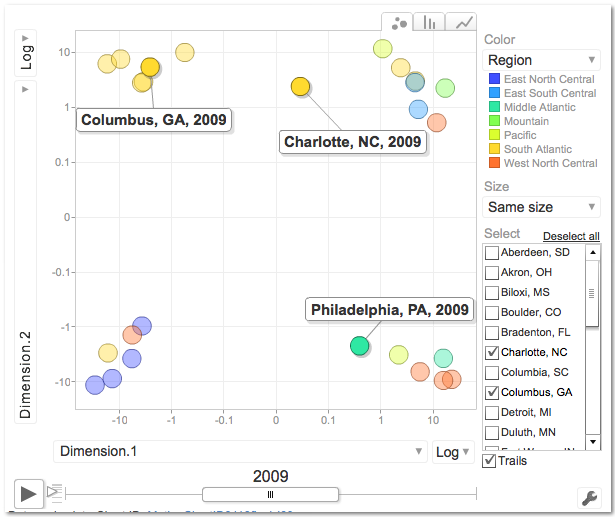
\includegraphics[width=\textwidth]{mdszscores09.png}
%\caption{2009}
\end{minipage}
\hspace{0.5cm}
\begin{minipage}[b]{0.45\linewidth}
\centering
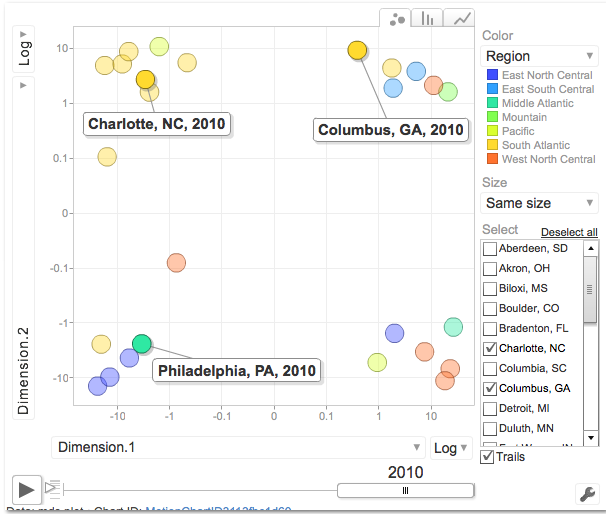
\includegraphics[width=\textwidth]{mdszscores10.png}
%\caption{2010}
\end{minipage}
\hspace{0.5cm}
\begin{minipage}[b]{0.45\linewidth}
\centering
%\includegraphics[width=\textwidth]{}
\caption{MDS results on the z-scores for
  2008-2010. Dimension 1 is on the x-axis and Dimension 2 is on the
  y-axis. The data are shown on the log-log scale, with color
  specified by Region.}
\label{fig:mdsMCzscores}
\end{minipage}
\end{framed}
\end{figure}

\pagebreak

Another way we can observe the differences between the communities is
to look at the results of average hierarchical cluster
analysis. This will not be discussed in detail here, but briefly
discussed in the 
Appendix. 

\section{Partial Least Squares Path Modeling}
The Knight Foundation identified social offerings, openness, and
aesthetics as the three main qualities that drive community
attachment. We explore these qualities by describing the directed
dependencies among these variables using Partial Least Squares Path
Modeling (PLSPM). PLSPM can be viewed as an extension of ordinary
least squares regression, in that the relationships among variables
can be analyzed by creating a system of interconnected linear
regressions through a network. Networks are comprised of latent and
manifest variables. Latent variables are those variables that cannot be directly
measured and are often determined by a combination of other variables,
while manifest variables are those variables that can be measured. 

The goal of PLSPM is to create an index for a latent variable, in this
case attachment. We will explore different networks for attachment
consisting of three latent variables: social offerings, openness, and
aesthetics. Viewing attachment as a function of social offerings,
openness, and aesthetics

\begin{equation}
Attachment = f(social \ \mathit{offerings}, openness, aesthetics)
\end{equation}

we aim to develop a model such that attachment can be determined by a
linear combination of latent variables: 

\begin{equation}
Attachment = \beta_{1}\mathit{Social.Offerings} + \beta_{2}Openness +
\beta_{3}Aesthetics
\end{equation}

Our hypothesis in each of the networks we modeled came from the
findings of the Knight Foundation: The better the quality of social
offerings, openness, and aesthetics, the higher the level of
attachment. 

We analyzed the 13 possible networks from these three latent variables
which are the index variables formed by the Knight Foundation. Figure
10 shows an example of one of the inner models: 

\begin{figure}[H]
\begin{center}
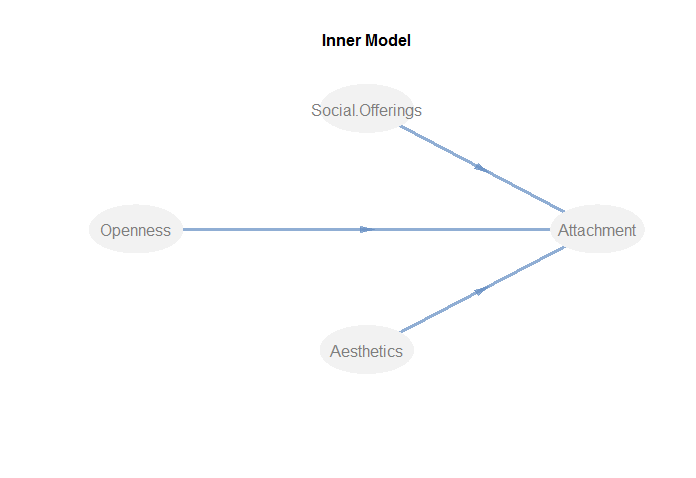
\includegraphics[width=\textwidth]{InnerModel.png}
\caption{Example of an inner model network.}
\label{fig:InnerModel}
\end{center}
\end{figure}



For our PLSPM analysis, we used as manifest variables (those variables
that can be measured) for social
offerings entertainment and places to meet, for openness welcoming,
and for aesthetics physical beauty and green places. Table
5 summarizes the variables used in our PLSPM
analysis from the questions in the Soul of the Community survey. 

\begin{table}[H]
\begin{center}
\begin{tabular}{P{3.cm}|P{3.cm}|P{5.5cm}}
\hline
\hline
Manifest Variable & Latent Variable & SOTC Survey Question \\
\hline
Entertainment venues & Social Offerings & Q7HR: Having a vibrant
nightlife with restaurants, clubs, bars, etc. \\
Places to meet & Social Offerings & Q7IR: Being a good place to meet
people and make friends \\
Welcoming & Openness & Q7MR: How much people care about each other \\
Physical beauty & Aesthetics & Q7BR: The beauty or physical setting \\
Green places & Aesthetics & Q7AR: The availability of outdoor parks,
playgrounds, and trails \\
Loyalty & Attachment & LOYALTY Index Variable \\
Passion & Attachment & PASSION Index Variable \\
\hline
\hline
\end{tabular}
\caption{Manifest and latent variables for PLSPM.}
\label{table:ManifestLatent}
\end{center}
\end{table}

\pagebreak

Figure 11 serves as an example of our outer model and
summarizes the variables used in our network models. 

\begin{figure}[H]
\begin{center}
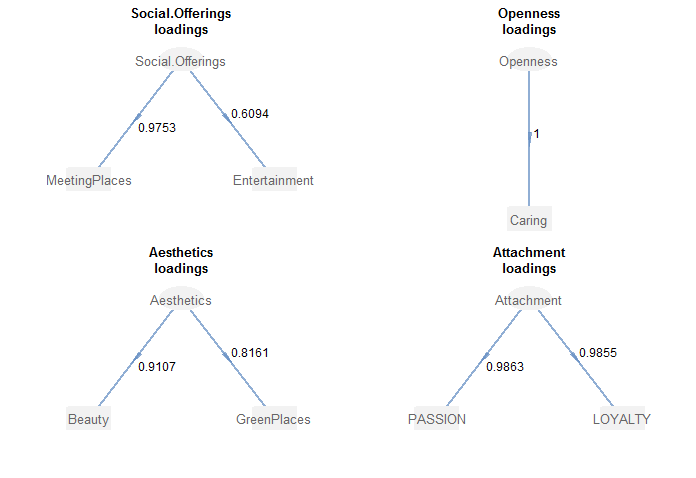
\includegraphics[width=\textwidth]{OuterModel.png}
\caption{Example of an outer model network.}
\label{fig:OuterModel}
\end{center}
\end{figure}

With the goal of analyzing the best model for attachment, we fit all
possible networks of latent variables for each year in the survey and
selected the top three based on the average overall goodness of fit by
year. The models with the highest average goodness of fit are shown in
the Figure 12. 

\begin{figure}[H]
\begin{framed}
\begin{minipage}[b]{0.45\linewidth}
\centering
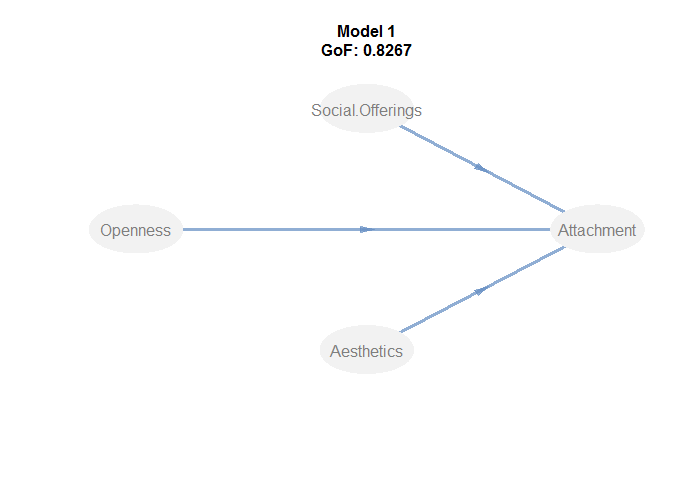
\includegraphics[width=\textwidth]{Mod1GoF.png}
%\caption{2008}
\end{minipage}
\hspace{0.5cm}
\begin{minipage}[b]{0.45\linewidth}
\centering
\includegraphics[width=\textwidth]{Mod2GoF.png}
%\caption{2009}
\end{minipage}
\hspace{0.5cm}
\begin{minipage}[b]{0.45\linewidth}
\centering
\includegraphics[width=\textwidth]{Mod3GoF.png}
%\caption{2010}
\end{minipage}
\hspace{0.5cm}
\begin{minipage}[b]{0.45\linewidth}
\centering
%\includegraphics[width=\textwidth]{}
\caption{Top three network models selected by goodness of fit.}
\label{fig:PLSPMtop3}
\end{minipage}
\end{framed}
\end{figure}


We applied the bootstrap procedure to assess the validity of the path
coefficients for each model. These 95\% bootstrap confidence intervals
for significant path coefficients are shown Figures
13-15 for each model. 

\begin{figure}[H]
\begin{framed}
\begin{minipage}[b]{0.45\linewidth}
\centering
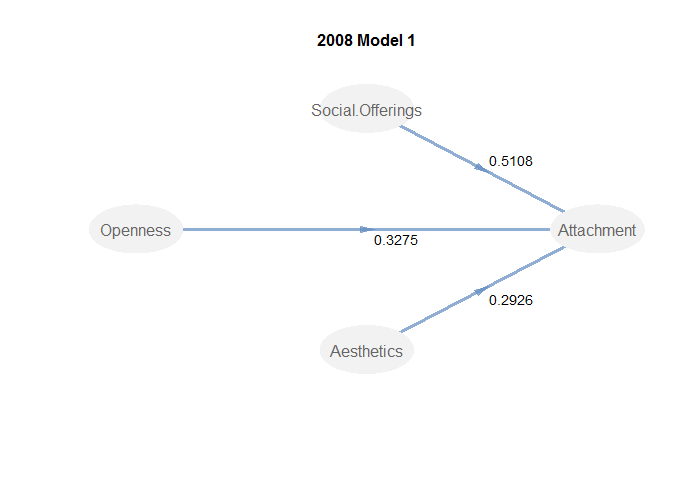
\includegraphics[width=\textwidth]{Mod12008.png}
%\caption{2008}
\end{minipage}
\hspace{0.5cm}
\begin{minipage}[b]{0.45\linewidth}
\centering
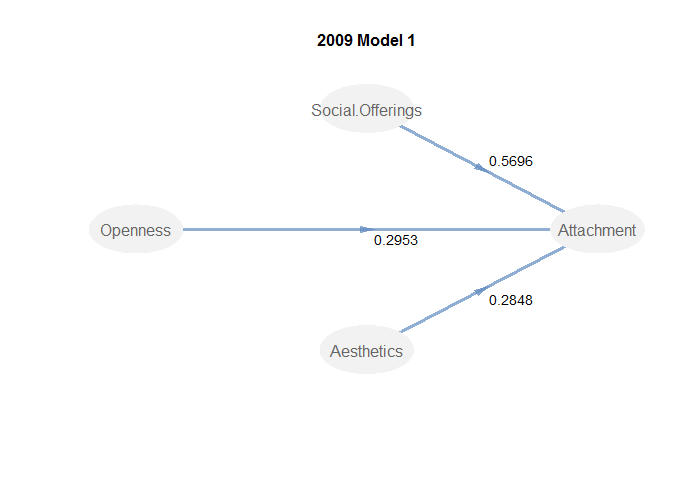
\includegraphics[width=\textwidth]{Mod12009.png}
%\caption{2009}
\end{minipage}
\hspace{0.5cm}
\begin{minipage}[b]{0.45\linewidth}
\centering
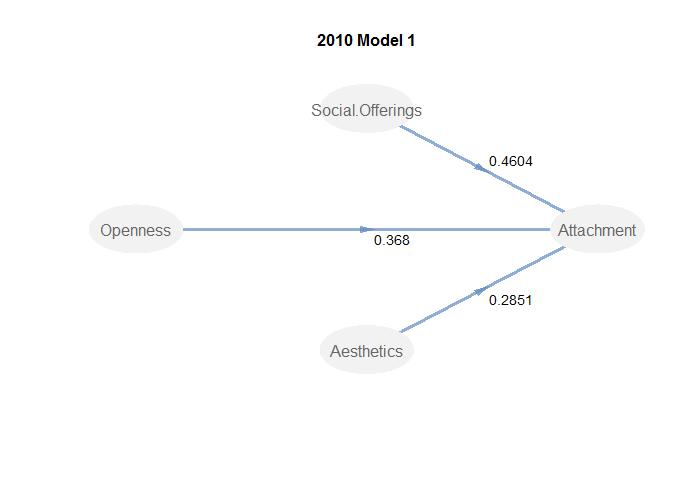
\includegraphics[width=\textwidth]{Mod12010.png}
%\caption{2010}
\end{minipage}
\hspace{0.5cm}
\begin{minipage}[b]{0.45\linewidth}
\centering
%\includegraphics[width=\textwidth]{}
\caption{Significant Coefficients: 
2008: Aesthetics (0.0701, 0.458)
2009: Social Offerings (0.290, 0.731)
      Openness (0.072, 0.404)
      Aesthetics (0.071, 0.452)
2010: Social Offerings (0.298, 0.681)
      Openness (0.187, 0.496)
      Aesthetics (0.022, 0.492).}
\label{fig:PLSPMmodel1}
\end{minipage}
\end{framed}
\end{figure}

\begin{figure}[H]
\begin{framed}
\begin{minipage}[b]{0.45\linewidth}
\centering
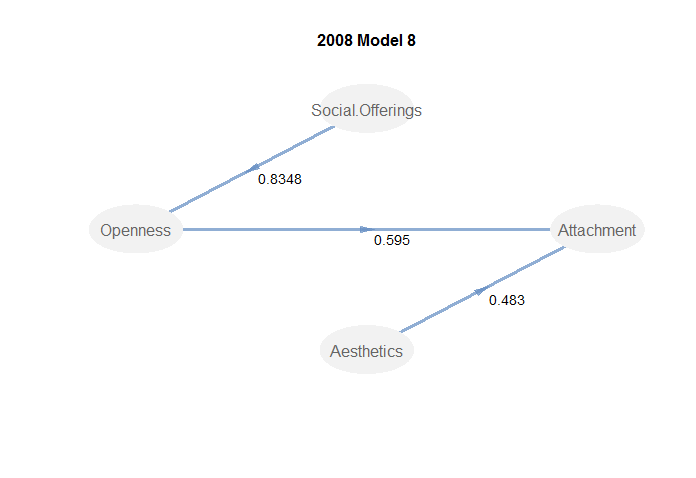
\includegraphics[width=\textwidth]{Mod22008.png}
%\caption{2008}
\end{minipage}
\hspace{0.5cm}
\begin{minipage}[b]{0.45\linewidth}
\centering
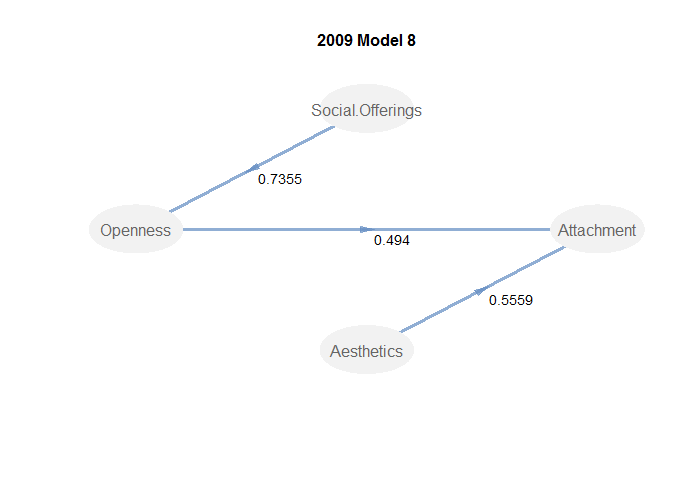
\includegraphics[width=\textwidth]{Mod22009.png}
%\caption{2009}
\end{minipage}
\hspace{0.5cm}
\begin{minipage}[b]{0.45\linewidth}
\centering
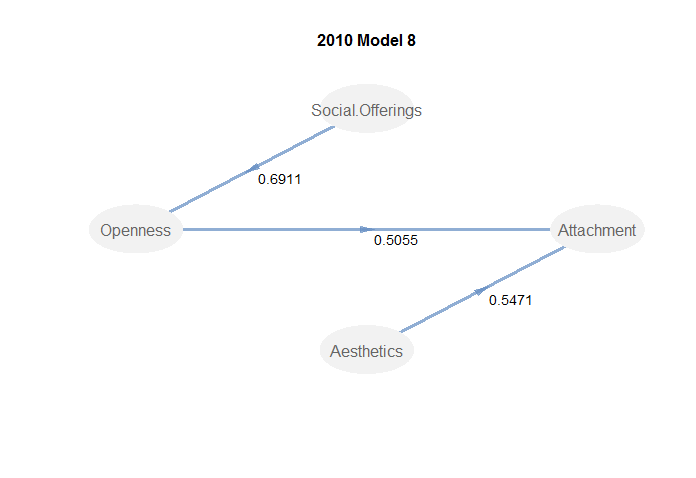
\includegraphics[width=\textwidth]{Mod22010.png}
%\caption{2010}
\end{minipage}
\hspace{0.5cm}
\begin{minipage}[b]{0.45\linewidth}
\centering
%\includegraphics[width=\textwidth]{}
\caption{Significant Coefficients: 
2008: Openness (0.388, 0.777)
      Aesthetics (0.288, 0.650)
2009: Openness (0.277, 0.633)
      Aesthetics (0.415, 0.690)
2010: Openness (0.333, 0.630)
      Aesthetics (0.394, 0.690).}
\label{fig:PLSPMmodel8}
\end{minipage}
\end{framed}
\end{figure}

\begin{figure}[H]
\begin{framed}
\begin{minipage}[b]{0.45\linewidth}
\centering
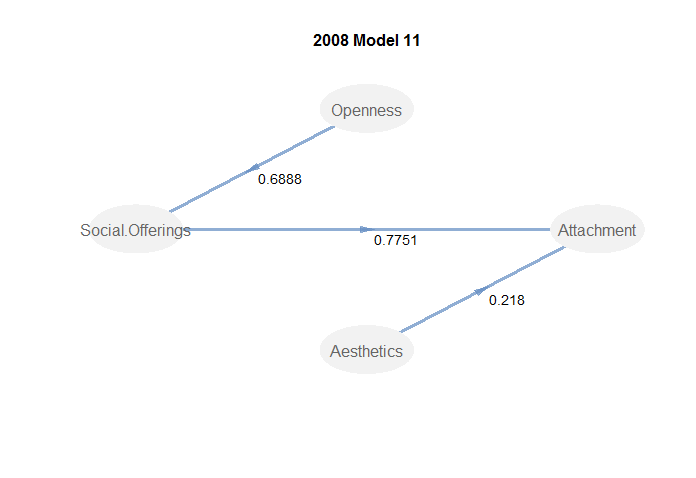
\includegraphics[width=\textwidth]{Mod32008.png}
%\caption{2008}
\end{minipage}
\hspace{0.5cm}
\begin{minipage}[b]{0.45\linewidth}
\centering
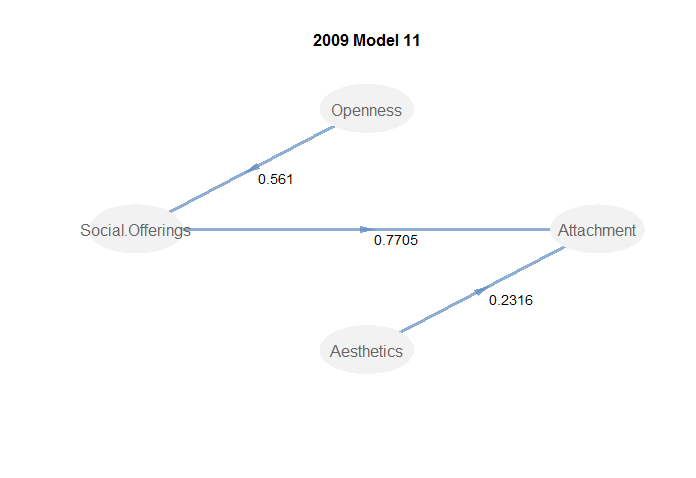
\includegraphics[width=\textwidth]{Mod32009.png}
%\caption{2009}
\end{minipage}
\hspace{0.5cm}
\begin{minipage}[b]{0.45\linewidth}
\centering
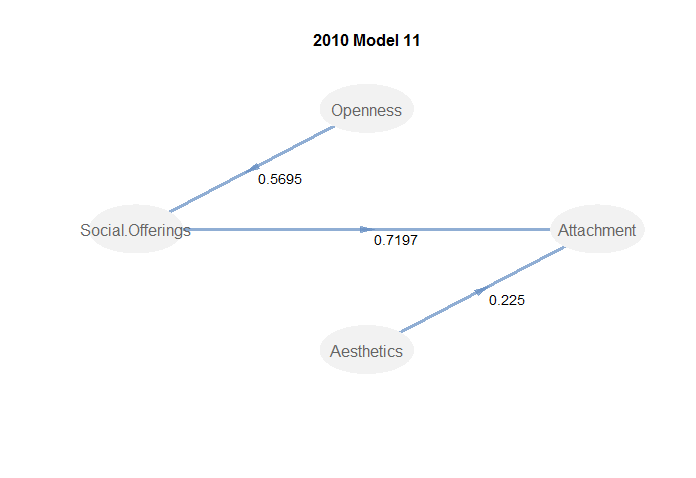
\includegraphics[width=\textwidth]{Mod32010.png}
%\caption{2010}
\end{minipage}
\hspace{0.5cm}
\begin{minipage}[b]{0.45\linewidth}
\centering
%\includegraphics[width=\textwidth]{}
\caption{Significant Coefficients: 
2008: Aesthetics (0.046, 0.412)
2009: Aesthetics (0.087, 0.477).}
\label{fig:PLSPMmodel11}
\end{minipage}
\end{framed}
\end{figure}

Based on the results of our PLSPM analysis, we find evidence to
support the findings of the Knight Foundation that the better the
quality of social offerings, openness, and aesthetics the higher the
level of attachment. Our best fitting model directly connects these
variables to attachment. Our second best model connects social
offerings indirectly to attachment through openness. This suggests
that having a vibrant social life with places to meet and make friends
creates a welcoming and caring environment that attaches people to
their communities. In contrast to our second model, our third best
model by goodness of fit indirectly connects openness to attachment
through social offerings. This model suggests that having a caring and
welcoming community promotes the development of places for people to
meet and make friends and as a result become attached to their
communities. 

\section{Conclusions and Future Research}
We have demonstrated the use of motion charts in displaying the results
of time-dependent multivariate analyses. Dynamic and interactive
interpretations can be achieved and customized based on the interest of
the user. Future research in this area will be to repeat the analyses
based on subsets of the data by the suggested clusters to further
understand the relationships between the index variables and cities, and
to better characterize what attaches people to their communities. In
addition, we aim to investigate the possibility of making the results
of our PLSPM analysis interactive.

\section{Acknowledgment}
The author greatly appreciates the generous comments and suggestions
of two anonymous reviewers on the first version of this article.

\pagebreak

\section{Appendix}
Tables 6-9 show the loadings from the MDS.

\begin{table}[H]
\begin{center}
\resizebox{8.65cm}{!}{
%\begin{tabular}{P{3.cm}P{1.5cm}P{1.5cm}P{1.5cm}|P{1.5cm}P{1.5cm}P{1.5cm}}
\begin{tabular}{P{3.75cm}{r}{r}{r}{r}{r}{r}}
\hline
\hline
& \multicolumn{3}{c}{Dimension 1} & \multicolumn{3}{c}{Dimension 2} \\
\hline
Index Variable & 2008 & 2009 & 2010 & 2008 & 2009 & 2010 \\
\hline
Aberdeen, SD & 0.54 & 0.56 & 0.46 & 0.19 &  -0.46 & -0.48 \\
Akron, OH & -0.50 & -0.49 & -0.53 & -0.06 & -0.02 & -0.04 \\
Biloxi, MS & 0.22 &  0.18 & 0.29 & 0.52 & -0.40 & 0.28 \\
Boulder, CO &  0.62 & 0.96 & 0.96 & -0.46 & 0.03 & -0.12 \\
Bradenton, FL &  0.23 & 0.64 & 0.56 & -0.28 & 0.34 & 0.22  \\
Charlotte, NC & 0.02 &  0.11 & 0.04 & 0.05 & 0.05 & 0.09 \\
Columbia, SC &  0.11 & 0.01 & -0.03 & 0.15 & 0.14 & 0.07 \\
Columbus, GA &  0.18 & 0.05 & 0.29 & 0.16 & 0.07 & 0.13 \\
Detroit, MI &  -1.29 & -1.42 & -1.42 & -0.10 & -0.24 & -0.08 \\
Duluth, MN &  0.42 & 0.43 & 0.39 & -0.30 & -0.04 & -0.18 \\
Fort Wayne, IN & -0.19 & -0.14 & 0.24 & 0.07 & 0.09 & 0.07 \\
Gary, IN & -1.63 &  -2.30 & -2.11 & 0.02 & -0.06 & -0.11 \\
Grand Forks, ND & 0.68 &  0.84 & 0.81 & 0.26 & -0.61 & -0.54 \\
Lexington, KY & 0.36 &  0.49 & 0.33 & 0.01 & 0.07 & -0.00 \\
Long Beach, CA & 0.23 & 0.27 & 0.38 &  0.06 & 0.18 & 0.21 \\
Macon, GA & -0.47 &  -1.20 & -1.23 & 0.10 & -0.02 & 0.04 \\
Miami, FL &  -0.86 & -0.87 & -0.85 & -0.30 & 0.37 & 0.23 \\
Milledgeville, GA & -0.13 & 0.02 & -0.74 & 0.14 & 0.10 & 0.07  \\
Myrtle Beach, SC &  0.36 & 0.41 & 0.27 & 0.29 & 0.34 & 0.37 \\
Palm Beach, FL &  -0.13 & 0.06 & 0.10 & -0.29 &  0.46 & 0.26 \\
Philadelphia, PA &  -0.18 & -0.18 & -0.35 & -0.01 & -0.13 & 0.01
\\
San Jose, CA &  0.19 & 0.14 & 0.14 & -0.08 & -0.08 & -0.09 \\
St. Paul, MN &  0.40 & 0.66 & 0.61 & -0.15 & -0.01 & -0.08 \\
State College, PA &  0.64 & 0.73 & 1.05 & -0.16 & -0.20 & -0.38 \\
Tallahassee, FL &  0.22 & 0.36 & 0.34 & -0.15 & 0.04 & -0.02 \\
Wichita, KS & -0.07 &  -0.36 & -0.02 & 0.31 & -0.02 & 0.04 \\
\hline
\end{tabular}}
\caption{Loadings for MDS on means for survey years 2008-2010}
\label{table:MDSmeans}
\end{center}
\end{table}


\begin{table}[H]
\begin{center}
\resizebox{8.65cm}{!}{
%\begin{tabular}{P{3.cm}P{1.5cm}P{1.5cm}P{1.5cm}|P{1.5cm}P{1.5cm}P{1.5cm}}
\begin{tabular}{P{3.75cm}{r}{r}{r}{r}{r}{r}}
\hline
\hline
& \multicolumn{3}{c}{Dimension 1} & \multicolumn{3}{c}{Dimension 2} \\
\hline
Index Variable & 2008 & 2009 & 2010 & 2008 & 2009 & 2010 \\
\hline
Aberdeen, SD & 0.18 & 0.12 & 0.27 & -0.07 & -0.08 & -0.04 \\
Akron, OH & -0.14 & -0.10 & -0.08 & -0.02 & -0.02 & 0.01 \\
Biloxi, MS &  -0.11 & -0.13 & -0.06 & -0.20 & -0.13 & -0.13 \\
Boulder, CO &  0.29 & 0.27 & 0.20 & 0.21 & 0.13 & 0.19 \\
Bradenton, FL & 0.05 & 0.18 & 0.16 & 0.05 & 0.02 & 0.01 \\
Charlotte, NC & -0.07 & -0.03 & -0.03 & 0.06 & -0.01 & 0.01 \\
Columbia, SC & 0.08 & 0.07 &  -0.05 & -0.02 & -0.05 & -0.00 \\
Columbus, GA & -0.05 & -0.11 & -0.08 & -0.14 & -0.12 & -0.19  \\
Detroit, MI & -0.34 & -0.23 & -0.25 & 0.06 & 0.09 & 0.03  \\
Duluth, MN &  0.22 &  0.06 & 0.00 & 0.12 & 0.13 & 0.11 \\
Fort Wayne, IN & -0.08 & 0.10 & 0.22 & -0.04 & 0.07 & 0.02 \\
Gary, IN & -0.40 & -0.37 & -0.46 & 0.18 & 0.12 & 0.11 \\
Grand Forks, ND & 0.12 & 0.19 & 0.27 & -0.11 & -0.14 & -0.12 \\
Lexington, KY & 0.23 & 0.19 & 0.10 & -0.06 & -0.02 & -0.01 \\
Long Beach, CA & 0.02 & 0.01 & 0.09 & -0.10 & -0.04 & -0.0 \\
Macon, GA & -0.28 & -0.40 & -0.41 & -0.14 & -0.01 & -0.03  \\
Miami, FL & -0.36 & -0.29 & -0.24 & 0.20 & 0.06 & 0.06 \\
Milledgeville, GA & -0.14 & -0.13 & -0.36 &  -0.10 & -0.09 &
-0.06 \\
Myrtle Beach, SC & 0.03 & -0.01 & 0.03 & -0.07 & -0.02 & 0.00 \\
Palm Beach, FL & -0.18 & 0.06 & -0.04 & 0.08 & 0.02 & -0.02 \\
Philadelphia, PA & -0.09 & 0.05 & -0.12 & 0.04 & 0.02 & 0.01 \\
San Jose, CA & 0.34 & 0.15 & 0.24 & -0.03 & 0.05 & 0.01 \\
St. Paul, MN & 0.16 & 0.20 & 0.21 & 0.02 & 0.06 & 0.05 \\
State College, PA & 0.39 & 0.20 & 0.30 & 0.04 & -0.01 & 0.00 \\
Tallahassee, FL &  0.04 & 0.05 & 0.06 & 0.00 & -0.01 & 0.03 \\
Wichita, KS & 0.08 & -0.11 & 0.02 & 0.02 & -0.00 & -0.02 \\
\hline
\end{tabular}}
\caption{Loadings for MDS on standard deviations for survey years
  2008-2010}
\label{table:MDSsd}
\end{center}
\end{table}

\pagebreak

\begin{table}[H]
\begin{center}
\resizebox{8.65cm}{!}{
%\begin{tabular}{P{3.cm}P{1.5cm}P{1.5cm}P{1.5cm}|P{1.5cm}P{1.5cm}P{1.5cm}}
\begin{tabular}{P{3.75cm}{r}{r}{r}{r}{r}{r}}
\hline
\hline
& \multicolumn{3}{c}{Dimension 1} & \multicolumn{3}{c}{Dimension 2} \\
\hline
Index Variable & 2008 & 2009 & 2010 & 2008 & 2009 & 2010 \\
\hline
Aberdeen, SD & 0.03 & -0.00 & 0.09 & 0.15 & 0.22 & 0.18 \\
Akron, OH &  0.10 & 0.10 & 0.15 & -0.07 & -0.05 & -0.08 \\
Biloxi, MS &  0.12 & 0.04 & 0.00 & 0.16 & 0.15 & 0.20 \\
Boulder, CO & -0.49 & -0.40 & -0.49 & -0.12 & -0.19 & -0.19 \\
Bradenton, FL &  -0.09 & -0.15 & -0.13 & 0.02 & 0.07 & -0.01  \\
Charlotte, NC & 0.05 &  0.03 & 0.06 & -0.02 & -0.01 & -0.03 \\
Columbia, SC & 0.06 &  0.06 & 0.09 & 0.01 & 0.02 & 0.02 \\
Columbus, GA & -0.00 & 0.03 & -0.02 & 0.07 & 0.10 & 0.13  \\
Detroit, MI & 0.14 &  0.17 & 0.23 &  -0.12 & -0.10 & -0.09 \\
Duluth, MN &  -0.23 & -0.17 & -0.23 & -0.06 & -0.12 & -0.11  \\
Fort Wayne, IN & 0.09 & 0.16 & 0.10 & -0.02 & -0.04 & -0.01 \\
Gary, IN & 0.22 & 0.26 & 0.29 & -0.14 & -0.13 & -0.08  \\
Grand Forks, ND & 0.01 & -0.10 & -0.15 & 0.25 & 0.24 & 0.22  \\
Lexington, KY & -0.02 & -0.01 & -0.01 & 0.01 & 0.03 & -0.00 \\
Long Beach, CA & -0.02 & 0.00 & 0.00 & 0.04 & 0.04 & 0.01 \\
Macon, GA & 0.10 & 0.16 & 0.20 & -0.03 & -0.04 & -0.02 \\
Miami, FL & 0.08 & 0.08 & 0.17 & -0.08 & -0.10 & -0.08  \\
Milledgeville, GA & 0.07 & 0.04 & 0.09 & 0.03 & 0.10 & 0.05 \\
Myrtle Beach, SC & -0.03 & -0.07 & 0.01 & 0.11 & 0.10 & 0.07 \\
Palm Beach, FL & -0.02 & -0.03 & -0.10 & -0.06 & -0.08 & -0.04  \\
Philadelphia, PA & 0.07 & 0.09 & 0.12 & -0.05 & -0.06 & -0.04 \\
San Jose, CA & 0.01 & 0.01 & 0.04 & -0.03 & -0.04 &  -0.06 \\
St. Paul, MN & -0.11 & -0.15 & -0.16 & -0.02 & -0.08 & -0.11 \\
State College, PA & -0.18 & -0.20 & -0.39 & 0.09 & 0.02 & 0.09 \\
Tallahassee, FL &  -0.10 & -0.11 & -0.09 & -0.06 & -0.05 & -0.05 \\
Wichita, KS & 0.13 & 0.14 & 0.12 & -0.02 & 0.00 & 0.03 \\
\hline
\end{tabular}}
\caption{Loadings for MDS on proportions for survey years 2008-2010}
\label{table:MDSproportions}
\end{center}
\end{table}

\begin{table}[H]
\begin{center}
\resizebox{8.65cm}{!}{
%\begin{tabular}{P{3.cm}P{1.5cm}P{1.5cm}P{1.5cm}|P{1.5cm}P{1.5cm}P{1.5cm}}
\begin{tabular}{P{3.75cm}{r}{r}{r}{r}{r}{r}}
\hline
\hline
& \multicolumn{3}{c}{Dimension 1} & \multicolumn{3}{c}{Dimension 2} \\
\hline
Index Variable & 2008 & 2009 & 2010 & 2008 & 2009 & 2010 \\
\hline
Aberdeen, SD & 14.87 & 15.83 & 18.52 & -9.76 & -9.45 & -11.30  \\
Akron, OH &  -9.26 & -5.67 & -5.79 & -5.94 & -3.77 & -4.35 \\
Biloxi, MS & 6.98 & 5.25 & 5.22 & 10.20 & 0.91 & 3.80  \\
Boulder, CO & 18.69 & 17.11 & 21.17 & 1.33 & 2.23 & 1.61  \\
Bradenton, FL & -2.72 & 2.42 & -0.45 & 5.88 & 5.25 & 5.49   \\
Charlotte, NC &  -0.79 & 0.02 & -2.87 & 3.35 & 2.39 & 2.71 \\
Columbia, SC & -0.15 & -3.67 & -2.39 & 2.98 & 2.78 & 1.60  \\
Columbus, GA & 1.54 & -2.54 & 0.38 & 4.88 & 5.38 &  9.26 \\
Detroit, MI & -16.11 & -13.46 & -13.69 & -10.42 & -8.74 & -9.67 \\
Duluth, MN & 9.22 & 5.66 & 7.56 & -5.91 & -6.56 & -3.36  \\
Fort Wayne, IN & -4.87 & -3.62 & 2.01 & -4.24 & -0.96 & -1.54 \\
Gary, IN & -26.36 & -28.76 & 23.42 & -11.64 & -11.45 & -14.14 \\
Grand Forks, ND & 21.51 & 22.82 & 23.30 & -10.83 & -9.01 & -6.83 \\
Lexington, KY & 4.61 & 4.54 & 1.88 & 1.37 & 2.81 & 1.89  \\
Long Beach, CA & 1.03 & 1.09 & -1.55 & 11.91 & 11.66 & 10.76 \\
Macon, GA & -8.48 & -16.20 & -20.06 & -0.84 & -2.97 & -2.44  \\
Miami, FL & -19.20 & -16.77 & -17.14 & 3.06 & 6.18 & 4.87  \\
Milledgeville, GA & -7.24 & -3.41 & -15.44 & 1.28 & 2.91 & 0.11  \\
Myrtle Beach, SC & -1.31 & -0.55 & -5.97 & 11.44 & 9.94 & 8.74 \\
Palm Beach, FL & -13.48 & -9.31 & -7.91 & 6.56 & 7.54 & 5.19 \\
Philadelphia, PA & -0.25 & 0.39 & -3.36 & -2.54 & -2.21 & -2.39 \\
San Jose, CA & 2.18 & 2.21 & 0.94 & -0.29 & -3.23 & -5.26  \\
St. Paul, MN & 10.30 & 11.81 & 11.23 & 0.83 & 0.52 & 2.12  \\
State College, PA & 18.99 & 15.76 & 26.78 & -4.21 & -3.72 & -1.18 \\
Tallahassee, FL & 3.19 & 4.61 & 1.78 & 2.74 & 2.99 & 4.39  \\
Wichita, KS & -2.89 & -5.58 & -0.73 & -1.19 & -1.40 & -0.08 \\
\hline
\end{tabular}}
\caption{Loadings for MDS on z-scores for survey years 2008-2010}
\label{table:MDSzscores}
\end{center}
\end{table}

\pagebreak

Hierarchical Cluster Analysis seeks to create clusters based on sets of
dissimilarities for the cities. Through the use of an iterative
algorithm, hierarchical cluster analysis begins with each city in
their own cluster, and then joins the cities together that are the
most similar. Figure 16 shows the dendrograms for each year, and the
clusters of cities obtained by this method. Cutting each tree at 0.8,
we can observe different numbers of clusters for each year, as well as
different groupings of the cities throughout time.


\begin{figure}[H]
\begin{framed}
\begin{minipage}[b]{0.45\linewidth}
\centering
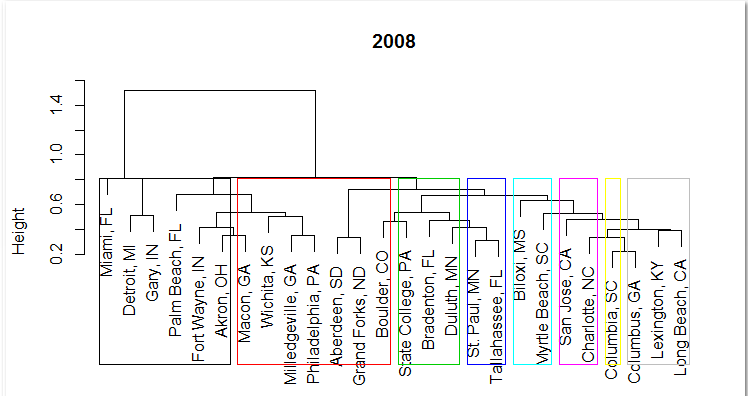
\includegraphics[width=\textwidth]{cluster08.png}
%\caption{2008}
\end{minipage}
\hspace{0.5cm}
\begin{minipage}[b]{0.45\linewidth}
\centering
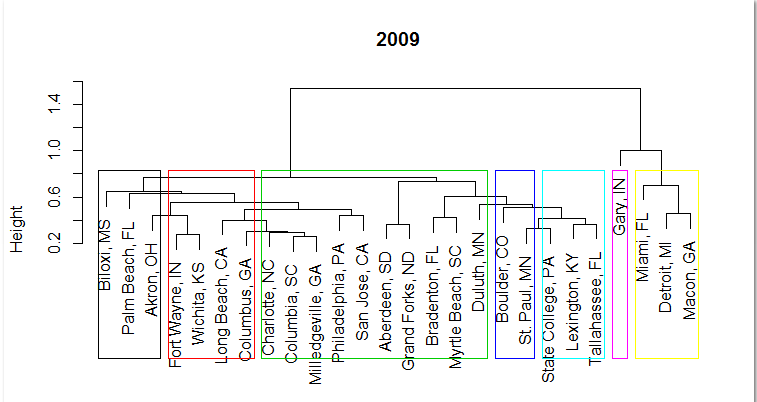
\includegraphics[width=\textwidth]{cluster09.png}
%\caption{2009}
\end{minipage}
\hspace{0.5cm}
\begin{minipage}[b]{0.45\linewidth}
\centering
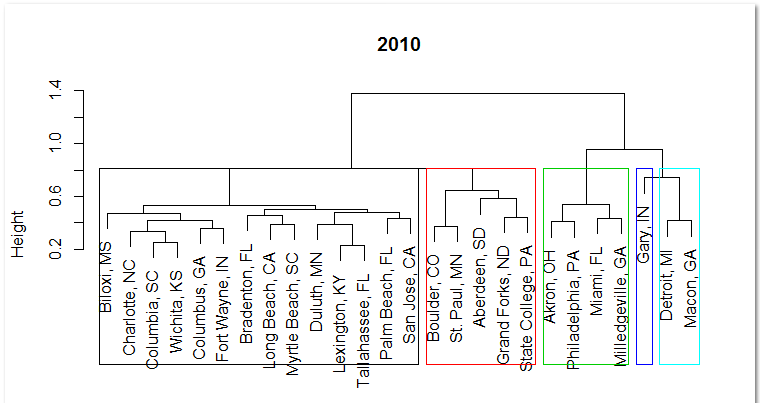
\includegraphics[width=\textwidth]{cluster10.png}
%\caption{2010}
\end{minipage}
\hspace{0.5cm}
\begin{minipage}[b]{0.45\linewidth}
\centering
%\includegraphics[width=\textwidth]{}
\caption{Average Hierarchical Cluster Analysis for survey years
  2008-2010.}
\label{fig:HCA}
\end{minipage}
\end{framed}
\end{figure}




%Note:BibTeX also works

\begin{references}
\itemsep=0pt
{\footnotesize
\item
Everitt, B. and Dunn, G. (2001), ``Applied Multivariate Data Analysis,''  {\it Hodder Arnold UK }.

\item 
Gesmann, M. and de Castillo, D. (2011), ``Using the Google
Visualization API with R,'' {\it The R Journal}, 3(2), 40--44.

\item
Hofmann, H., Wickham, H., Cook, D. (2019) The 2013 Data Expo of the American Statistical Association, Computational Statistics XX(YY):This Issue.

\item 
Husson, F., Josse, J., Le, S. and Mazet, J. (2013), {\it R package
  version 1.24. http://CRAN.R-project.org/package=FactoMineR}.

\item 
Knight Foundation Soul of the Community (2013), 
{\it What Attaches People to Their Communities?}
 {\it http://www.soulofthecommunity.org/}.

\item 
R Core Team (2013), ``R: A language and environment for statistical
computing,'' {\it R Foundation for Statisticcal Computing, Vienna,
  Austria http://www.R-project.org/}.

\item 
Wickham, H. (2009), ``\texttt{ggplot2}: elegant graphics for data
analysis,''  {\it Springer New York }.

\item
Sanchez, G. (2013). ``LS Path Modeling with R.'' Trowchez
Editions. Berkely, 2013. \\
{\it http://www.gastonsanchez.com/PLSPathModelingwithR.pdf} 

}
\end{references}


\end{document}


